\documentclass[a4paper, 12pt]{article}
\usepackage[T2A,T1]{fontenc}
\usepackage[utf8]{inputenc}
\usepackage[english, russian]{babel}
\usepackage{graphicx}
\usepackage[hcentering, bindingoffset = 10mm, right = 15 mm, left = 15 mm, top=20mm, bottom = 20 mm]{geometry}
\usepackage{multirow}
\usepackage{lipsum}
\usepackage{mathrsfs}
\usepackage{amsmath, amstext}
\usepackage{siunitx}
\usepackage{subcaption}
\usepackage{wrapfig}
\usepackage{adjustbox}
\usepackage{enumerate, indentfirst, float}
\usepackage{capt-of, svg}
\usepackage{icomma}

\newenvironment{bottompar}{\par\vspace*{\fill}}{\clearpage}

\begin{document}
	\begin{titlepage}
		
		\newcommand{\HRule}{\rule{\linewidth}{0.5mm}} % Defines a new command for the horizontal lines, change thickness here
		
		\center % Center everything on the page
		
		%----------------------------------------------------------------------------------------
		%	HEADING SECTIONS
		%----------------------------------------------------------------------------------------
		
		\textsc{\LARGE Московский \\[0.5cm] Физико-Технический Институт}\\[1,5cm] % Name of your university/college
		\textsc{\Large Кафедра общей физики}\\[0.5cm] % Major heading such as course name
		\textsc{\large Лабораторная работа \textnumero  3.4.5}\\[0.5cm] % Minor heading such as course title
		
		%----------------------------------------------------------------------------------------
		%	TITLE SECTION
		%----------------------------------------------------------------------------------------
		
		\HRule
		\\[0.4cm]
		{ \huge \bfseries Петля гистерезиса \\(динамический метод)}
		\\[0.2cm] % Title of your document
		\HRule
		\\[1.5cm]
		
		%----------------------------------------------------------------------------------------
		%	AUTHOR SECTION
		%----------------------------------------------------------------------------------------
		
		%\begin{minipage}{0.4\textwidth}
		\begin{flushleft} \large
			\emph{Студент:}\\
			Павел \textsc{Северилов} \\
			671 группа
		\end{flushleft}
		%\end{minipage}
		
		\begin{bottompar}
			\begin{center}
				
\includegraphics[width = 80 mm]{logo.jpg}
			\end{center}
			{\large \today}
			
		\end{bottompar}
		\vfill % Fill the rest of the page with whitespace
		
	\end{titlepage}

\section{Цель работы} Исследование петель гистерезиса ферромагнитных материалов с помощью осциллографа.

\textbf{В работе используются:} \textit{понижающий трансформатор, реостат, амперметр и вольтметр (мультиметры), резистор, делитель напряжения, интегрирующая цепочка, электронный осциллограф, тороидальные образцы с двумя обмотками.}
	
\section{Теоретическая часть}		 
	Магнитную индукцию удобно определять с помощью ЭДС, возникающей при изменении магнитного потока $\Phi$ в катушке, намотанной на образец: $~~\mathscr{E}=-\frac{d\Phi}{dt}$.
	
	Пусть катушка плотно обхватывает образец, и индукция $\textbf{B}$
	в образце однородна. Тогда $\Phi=BSN$, где $N$ - число витков в измерительной катушке, а $S$ -- число витков.
	Подставим $\Phi$ в формулу ЭДС, после интегрирования найдем:
	$$|B|=\frac{1}{SN}\int\mathscr{E} dt$$
	
	Таким образом, для определения $B$ нужно проинтегрировать сигнал, наведенный меняющимся магнитным полем на измерительную катушку, намотанную на образец.
	
	Для интегрирования сигнала применяют интегрирующие схемы. На рис.1 изображена простейшая из них. При этом сопротивление $R$ заметно превышает сопротивление конденсатора ($U_{\text{вых}}\ll U_{\text{вх}}$).
		
	\begin{center}
	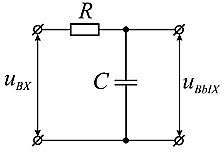
\includegraphics[width = 0.3\textwidth]{pic1.png}
	\end{center}
	
	В данном случае $I \approx U_{\text{вх}}/R$, а напряжение на емкости $$U_{\text{вых}}=\cfrac{q}{C}=\frac{1}{C}\int Idt \approx \cfrac{1}{RC}\int U_{\text{вх}}dt$$
	
	Чем больше постоянная времени $\tau =RC$ превосходит характерное время процесса, тем этот вывод ближе к истине. Для синусоидальных напряжений $U${\scriptsize вых}$=U${\scriptsize вх}$/RC\Omega$, где $\Omega$ - частота сигнала.
	
	Обозначив параметры интегрирующей ячейки через $R_{\text{и}}, C_{\text{и}}, N_{\text{и}}$, получим: $$|B|=\cfrac{R_{\text{и}}C_{\text{и}}}{SN_{\text{и}}}U_{\text{вых}}$$

\newpage

\section{Экспериментальная установка}

Ток в обмотке $N_0$ измеряется мультиметром А. Напряжение с сопротивления $R_0$, включенного последовательно с обмоткой $N_0$, подается на вход $X$ электронного осциллографа (ЭО). Это напряжение пропорционально току в обмотке $N_0$, а следовательно, и напряженности $H$ магнитного поля в образце. 

Для измерения магнитной индукции $B$ с измерительной обмотки $N_i$ на вход интегрирующей $NC$-цепочки подается напряжение $U_{BX}$, пропорциональное производной $B$, а с выхода снимается напряжение $U_{EX}=U_C$, пропорциональное $B$ и подается на вход $Y$.

Замкнутая кривая, возникающая на экране, воспроизводит в некотором масштабе (различном для $X$ и $Y$) петлю гистерезиса.Необходимо провести калибровку каналов $X$ и $Y$ ЭО и установить масштабы изображения. Для этого надо узнать, каким напряжениям (или токам) соответствуют амплитуды сигналов, видимых на экране, и каким значениям $B$ и $H$ соответствуют напряжения (или токи).
\begin{center}
	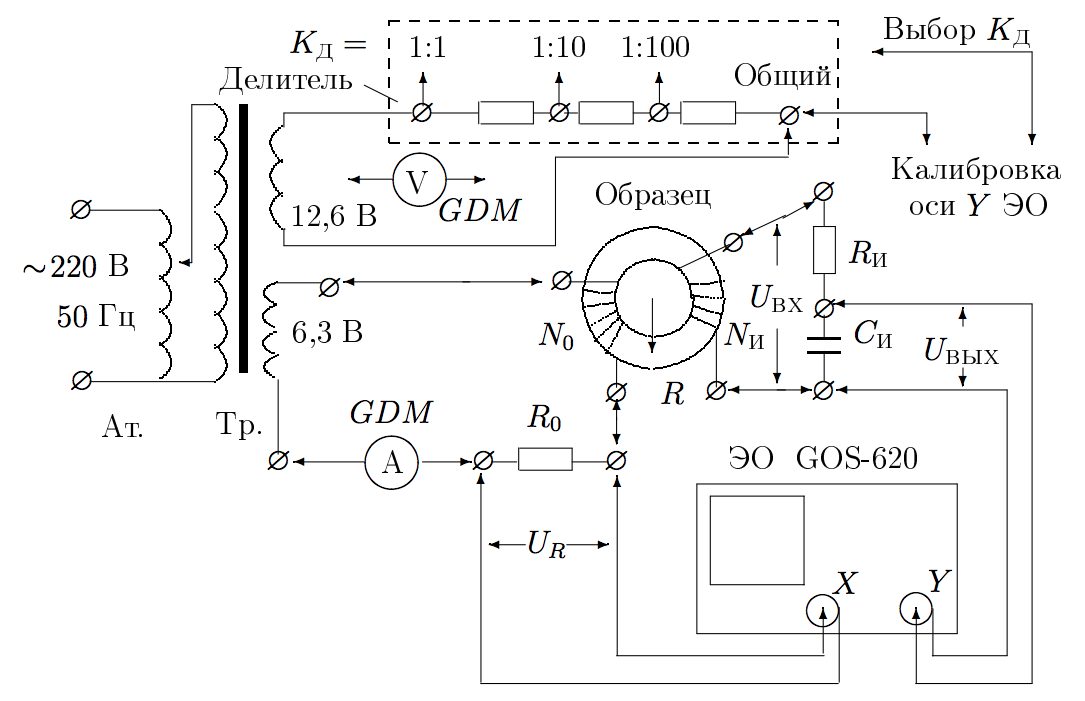
\includegraphics[width = 0.8\textwidth]{345-1.png}
\end{center}\
\textbf{Для измерения напряжения с помощью осциллографа:}
$$
2U_{X,0}=2x\cdot K_X; \hspace{2cm} 2U_{Y,0}=2y\cdot K_Y; \hspace{2cm} H=\frac{IN_0}{2\pi R}
$$
$$
|B|=\frac{R_uC_u}{SN_u}U_{ex}
$$

\textbf{Проверка калибровки горизонтальной оси ЭО с помощью амперметра:} (при закороченной обмотке $N_0$) 
$$
m_X=2R_0\sqrt{2}I_{ef}/(2x) 
$$
\textbf{Проверка калибровки вертикальной оси ЭО с помощью вольтметра:} (при отключенном тороиде)
$$
m_Y=2\sqrt{2}U_{ef}/(2y) 
$$
\textbf{Для измерения постоянной времени $RC$-цепочки:}
$$
\tau=RC=\frac{U_{in}}{\Omega U_{ex}}
$$

\bigskip


\section{Работа и измерения}
\begin{center}
\textbf{1. Петля гистерезиса на экране ЭО}
\end{center}

Соберем схему согласно рисунку выше, подготовим приборы к работе и включим схему в сеть. Подберем ток питания в намагничивающей обмотке и коэффициенты усиления ЭО, так, чтобы предельная петля гистерезиса занимала большую часть экрана, но при этом исчезли "усы". Проверим центровку вертикальных и горизонтальных лучей.

Для каждого материала зафиксируем предельную петлю и снимем начальную кривую намагничивания, плавно уменьшая ток до нуля и отмечая вершины наблюдаемых частных петель. Затем восстановим предельную петлю, измерим на экране двойные амплитуды для коэрцитивной силы $[2x(c)]$ и индукции насыщения $[2y(s)]$. Запишем соответствующие значения $K_x$ и $K_y$.

Параметры схемы:$~~R_0=0,3\text{ Ом};~~R_u=20\text{ кОм}~~~C_u=20\text{ мкФ}$
\begin{table}[H]
	\centering
\begin{tabular}{|c|c|c|c|}
	\hline 
	 &Пермаллой& Феррит&Кремнистое железо \\ \hline 
	$K_X$, мВ/дел & 20&10&20  \\ \hline
	$K_Y$, мВ/дел & 50&10&50 \\ \hline
	$I_{ef},$ мA &234,5  &117&234\\ \hline
	$2\pi R,$ см & 24 &25&10\\ \hline
	$N_0,$витков & 35 &40&40\\ \hline
	$N_U,$витков & 220 &400&400\\ \hline
	$S, \text{см}^2$ & 3,8 &3,0&1,2\\ \hline
	$2x(c),$ делений& 6,6&7&10\\ \hline
	$2y(s),$ делений& 8&6&5,2\\ 	\hline
\end{tabular}
\caption{Данные для трех ферромагнетиков}
\end{table}


\begin{center}
	\textbf{Пермаллой}
\end{center}

\begin{figure}[h]
	\begin{minipage}[h]{0.5\linewidth}
		\center{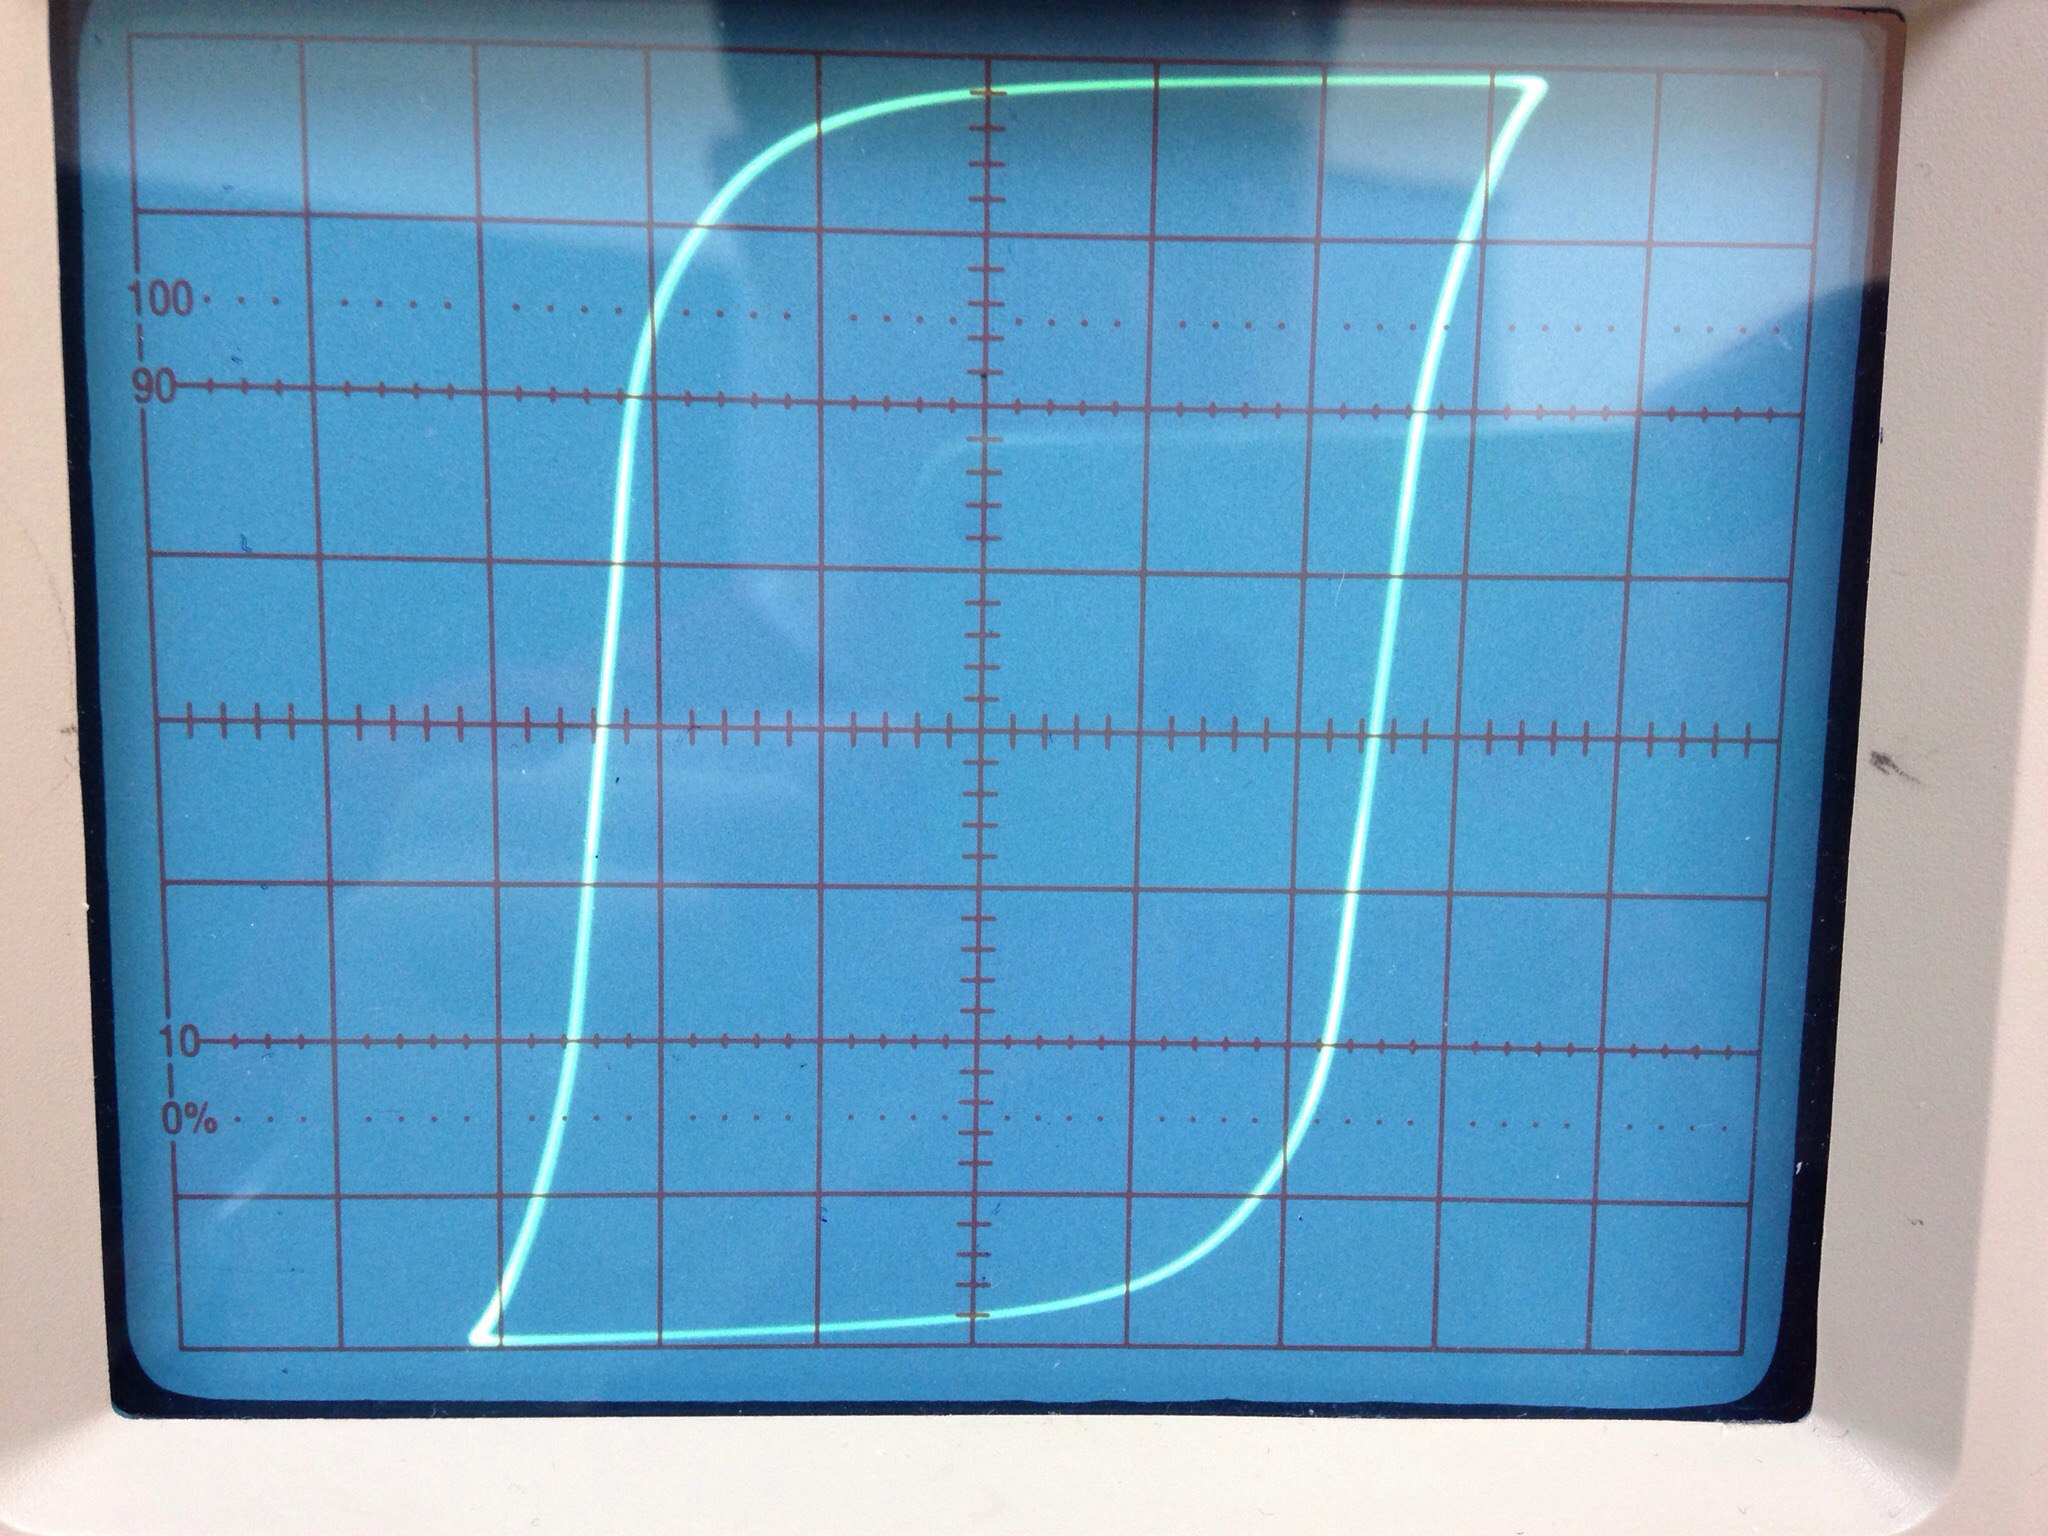
\includegraphics[width=\linewidth]{Fe-Ni}}\\ предельная петля
	\end{minipage}
	\begin{minipage}[h]{0.5\linewidth}
		\center{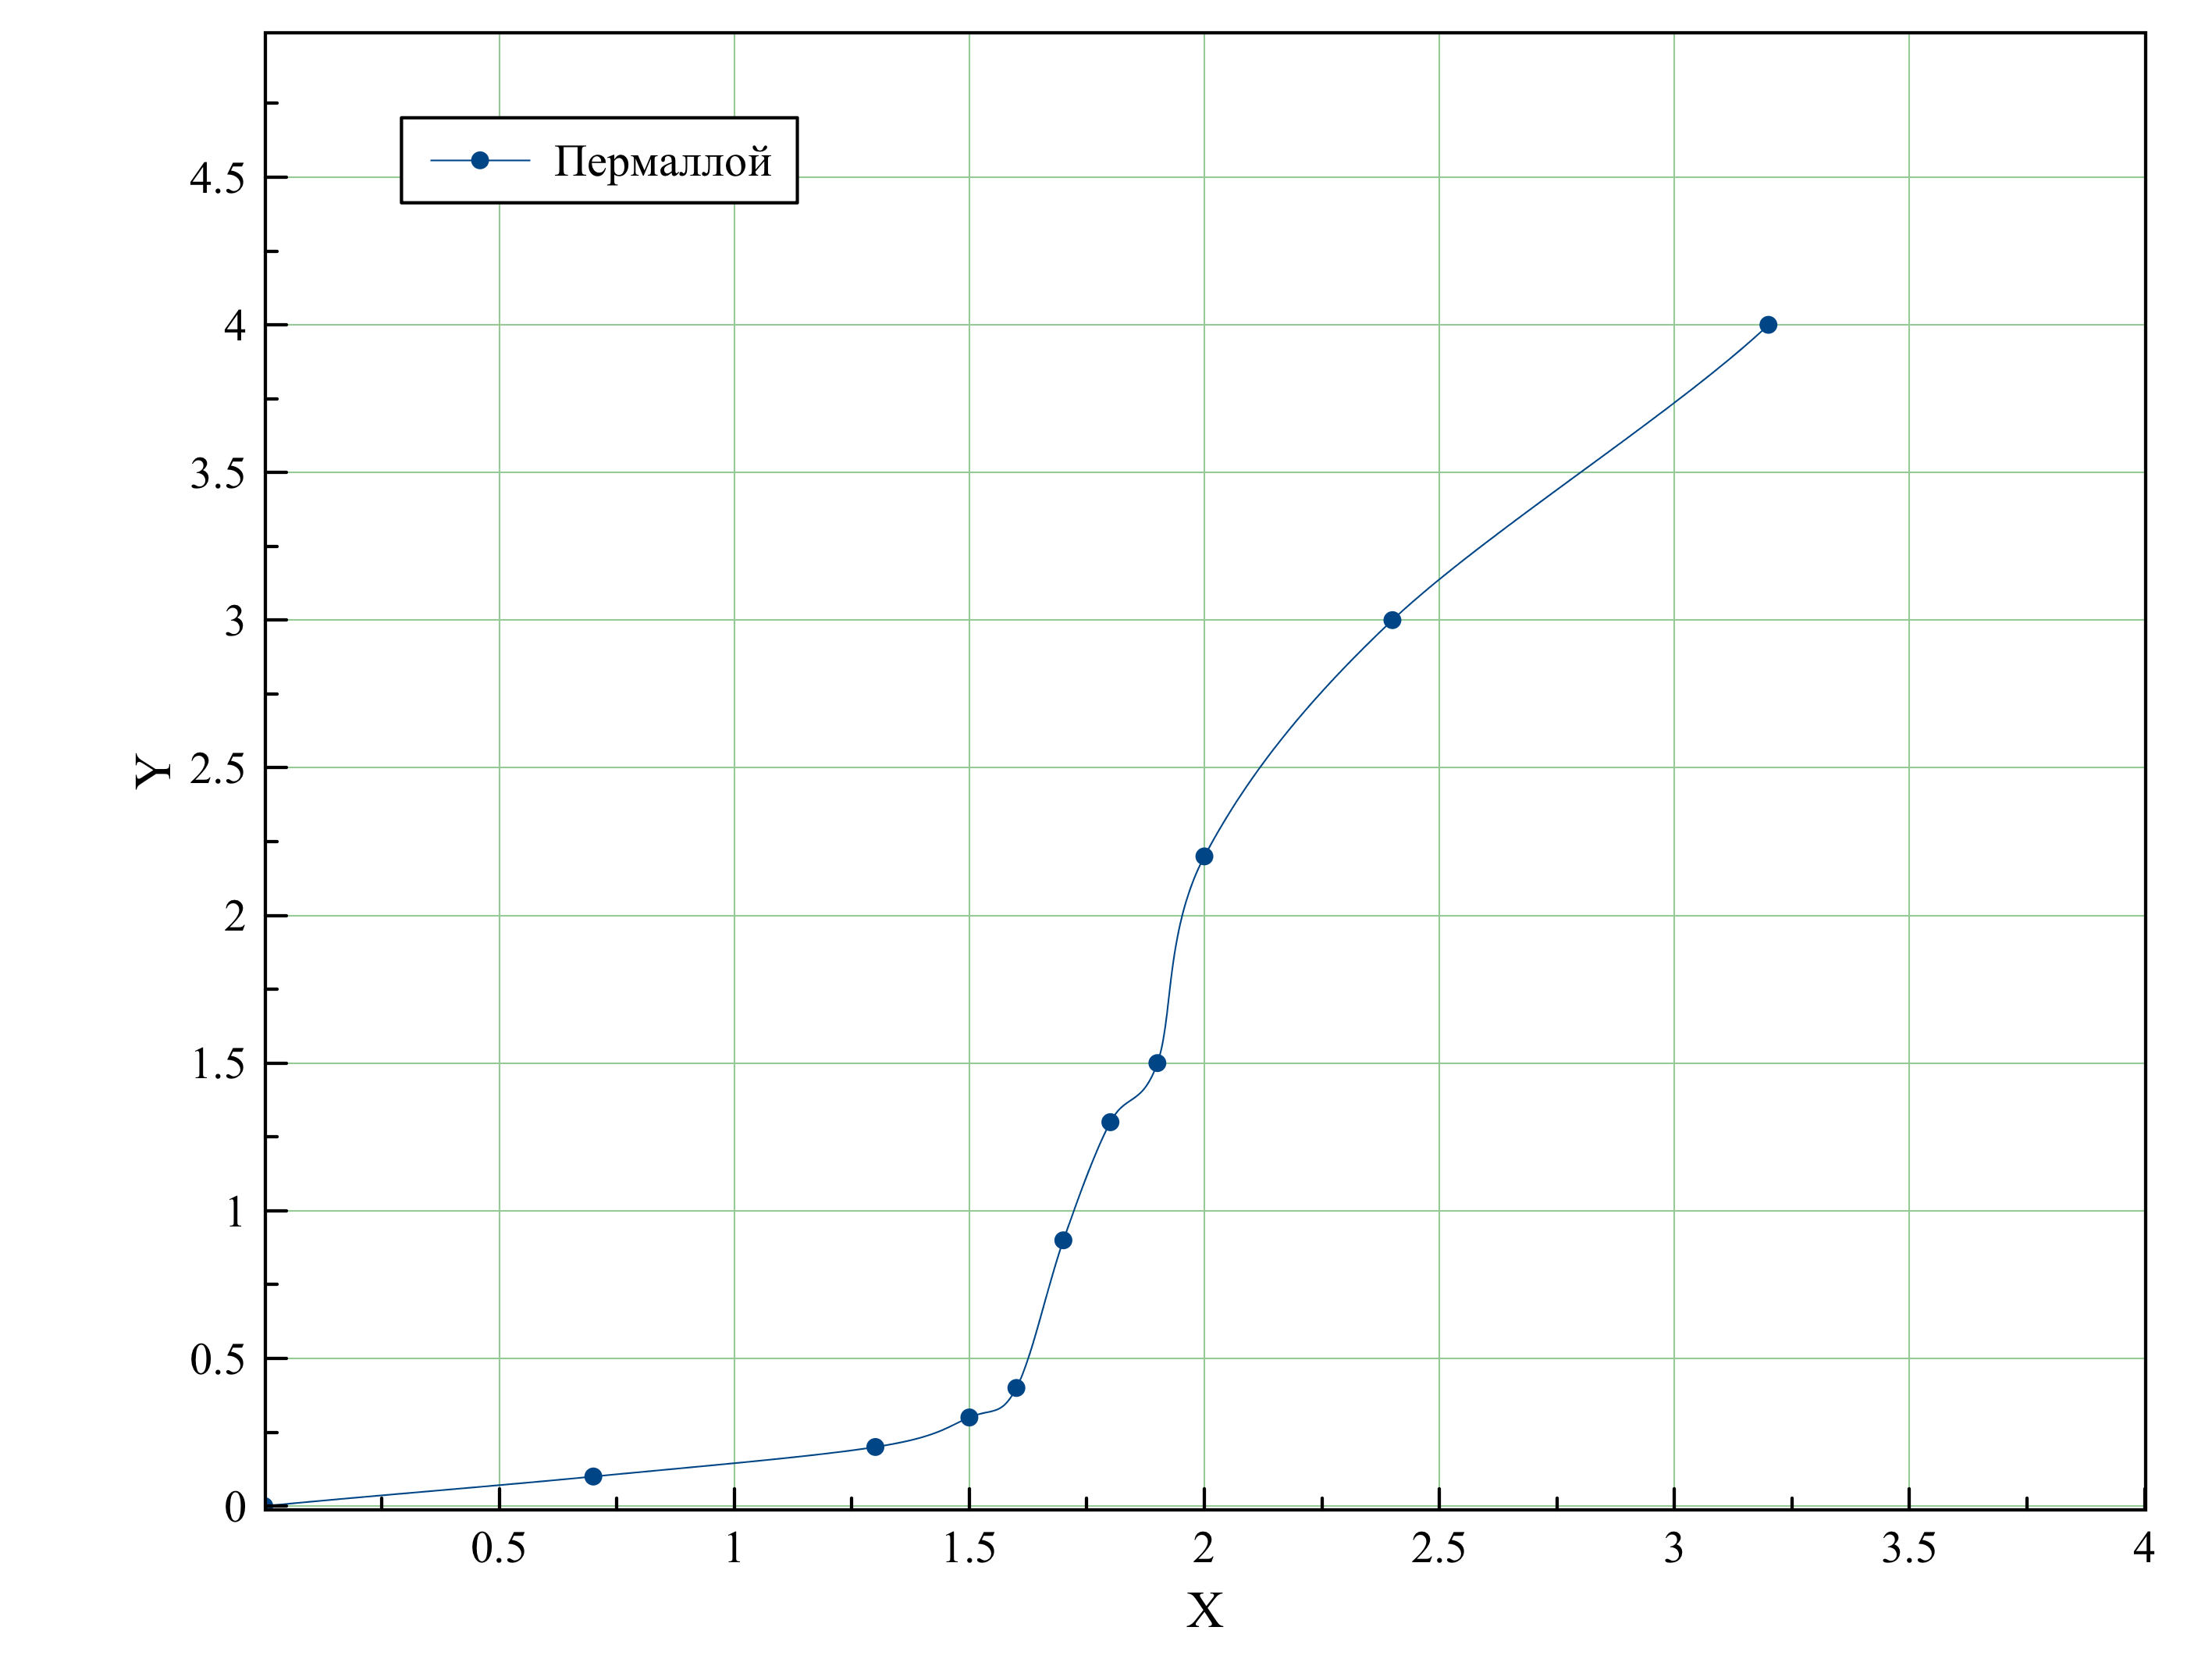
\includegraphics[width=\linewidth]{Fe-Ni_plot}}\\ начальная кривая
	\end{minipage}
\end{figure}

\newpage

\begin{center}
	\textbf{Феррит}
\end{center}

\begin{figure}[h]
	\begin{minipage}[h]{0.5\linewidth}
		\center{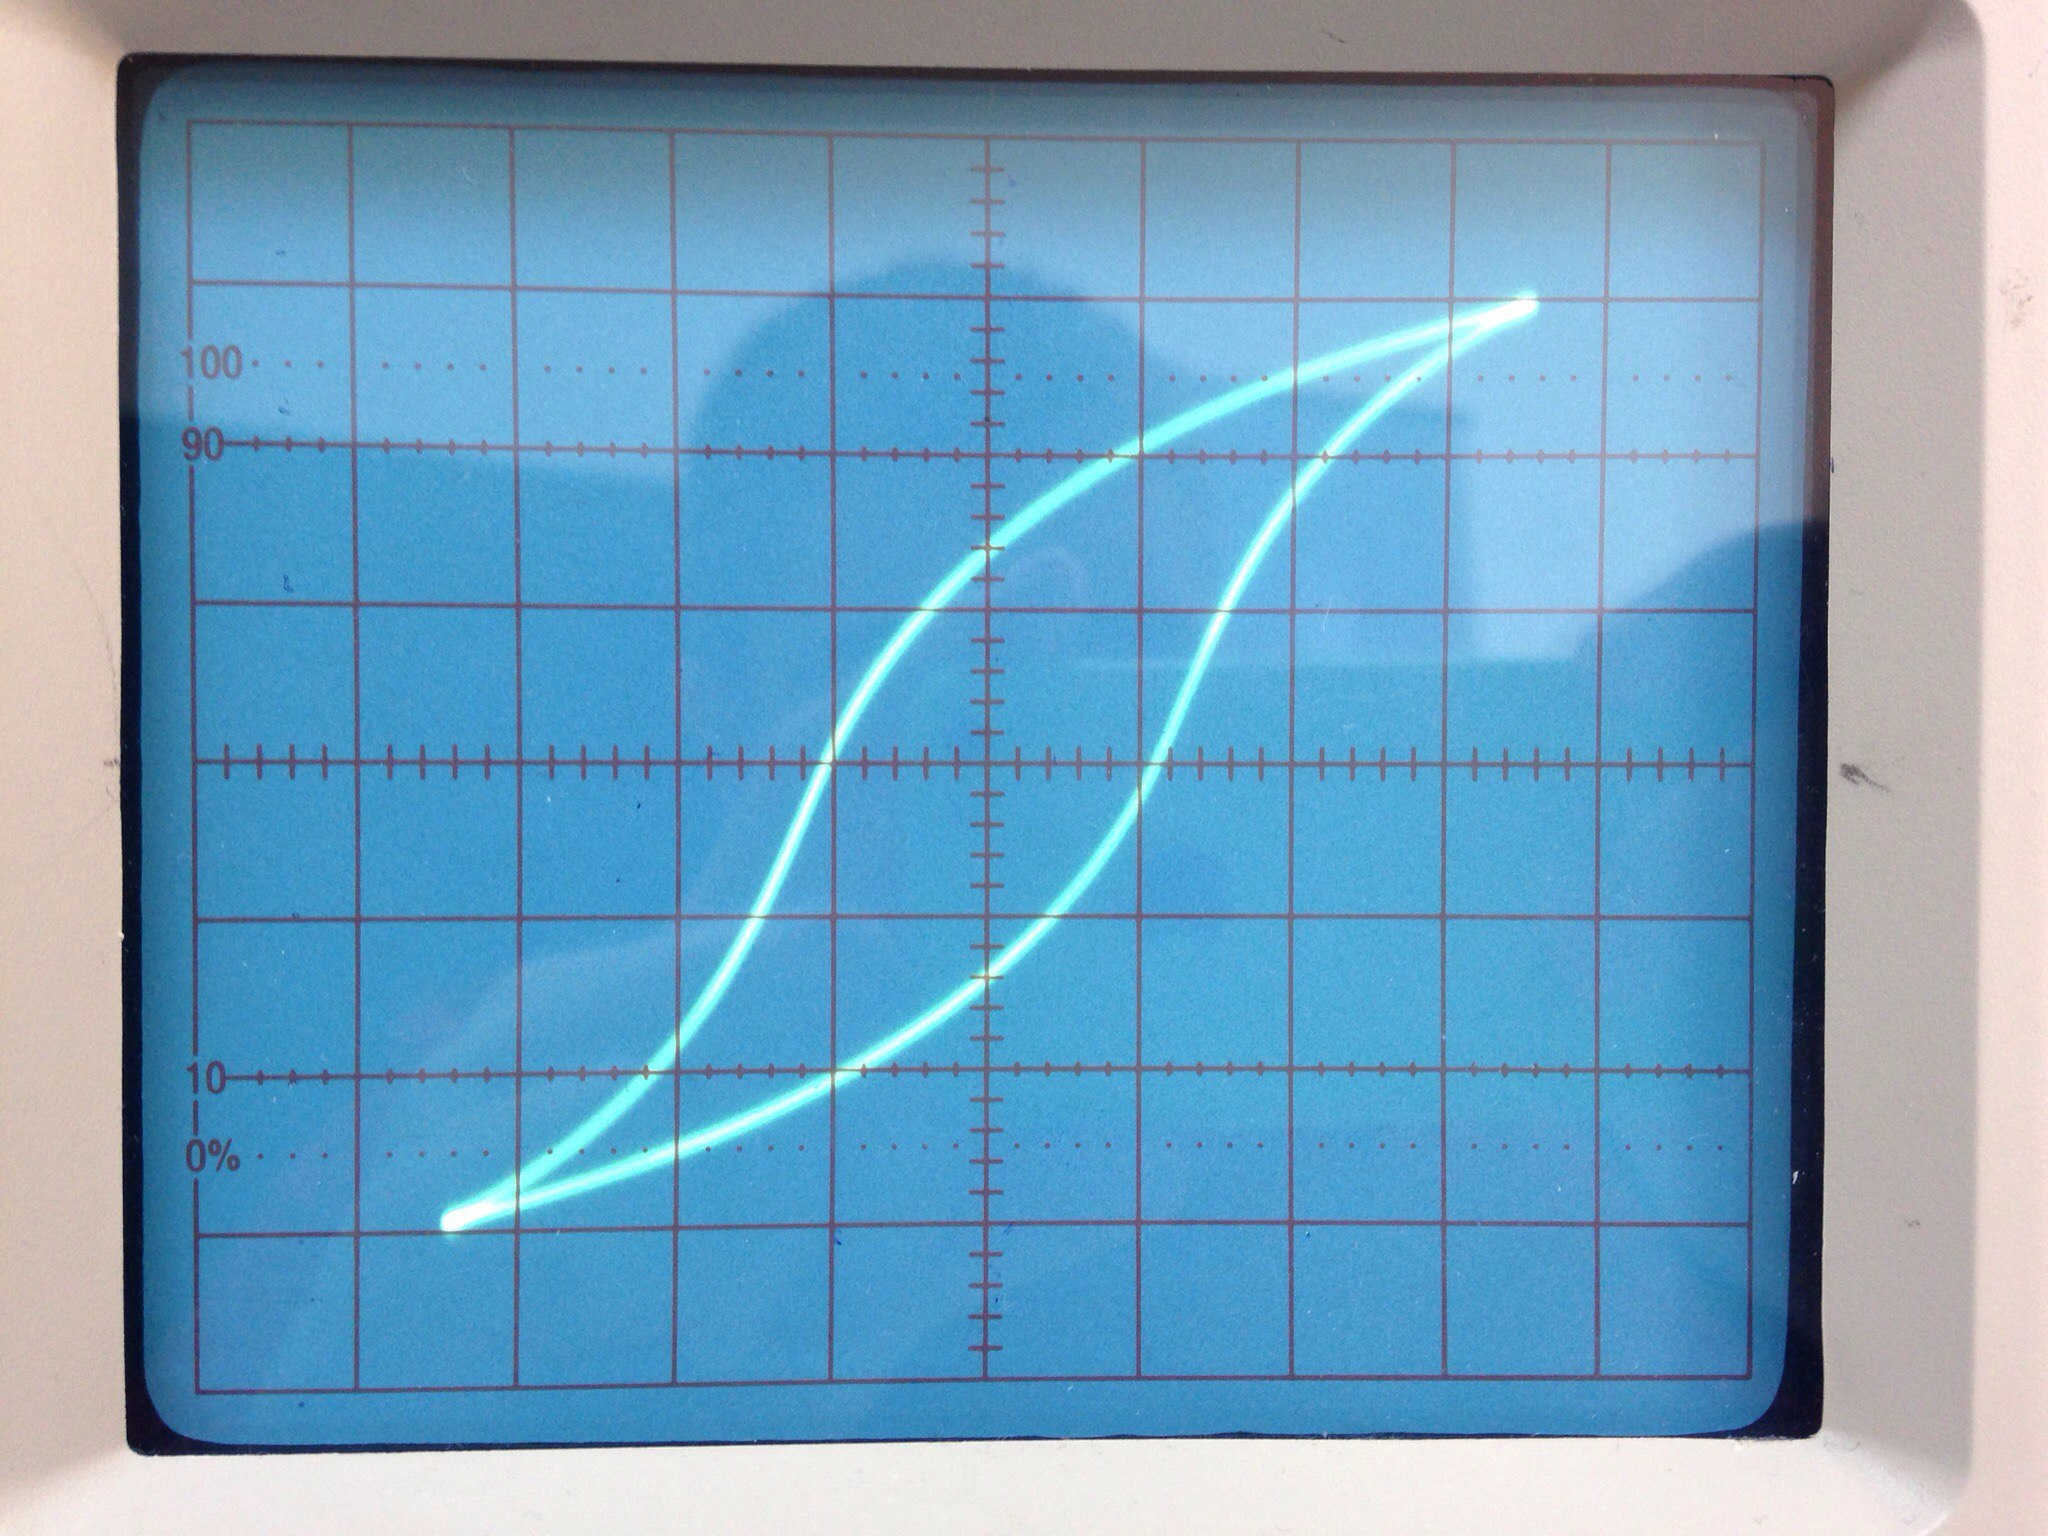
\includegraphics[width=\linewidth]{Ferrit}}\\ предельная петля
	\end{minipage}
	\begin{minipage}[h]{0.5\linewidth}
		\center{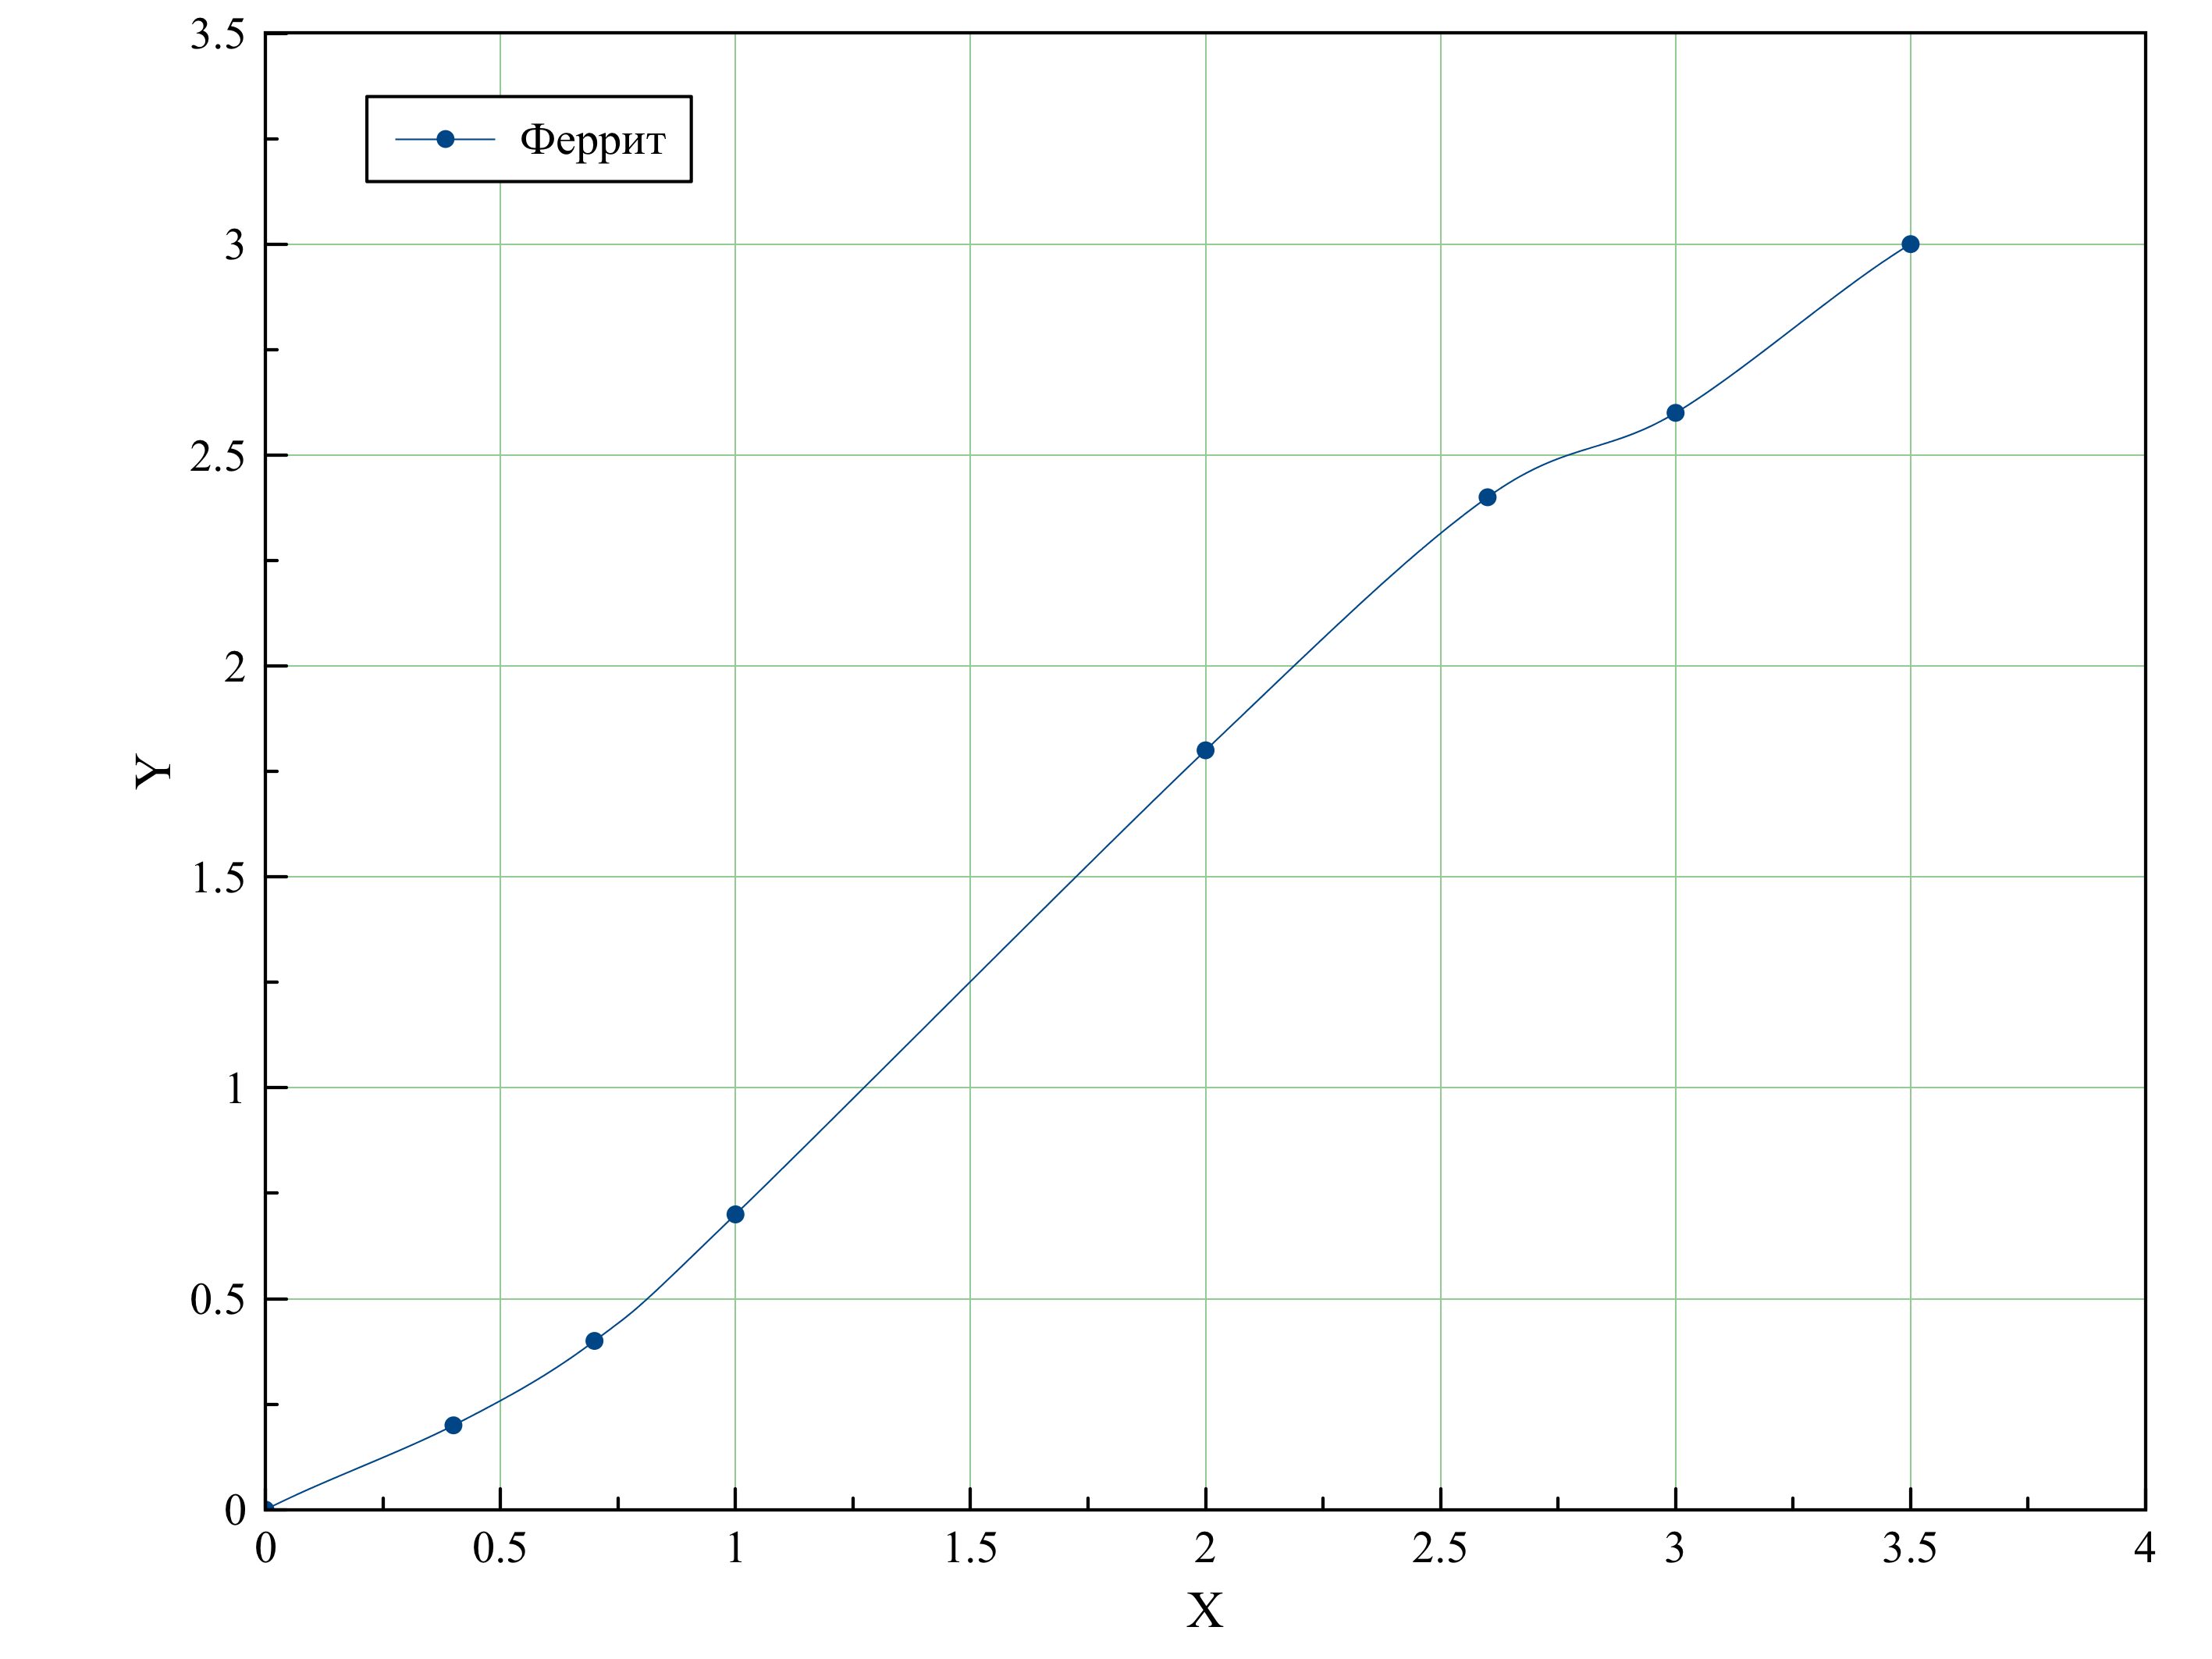
\includegraphics[width=\linewidth]{Ferrit_plot}}\\ начальная кривая
	\end{minipage}
\end{figure}

\begin{center}
	\textbf{Кремнистое железо}
\end{center}

\begin{figure}[h]
	\begin{minipage}[h]{0.5\linewidth}
		\center{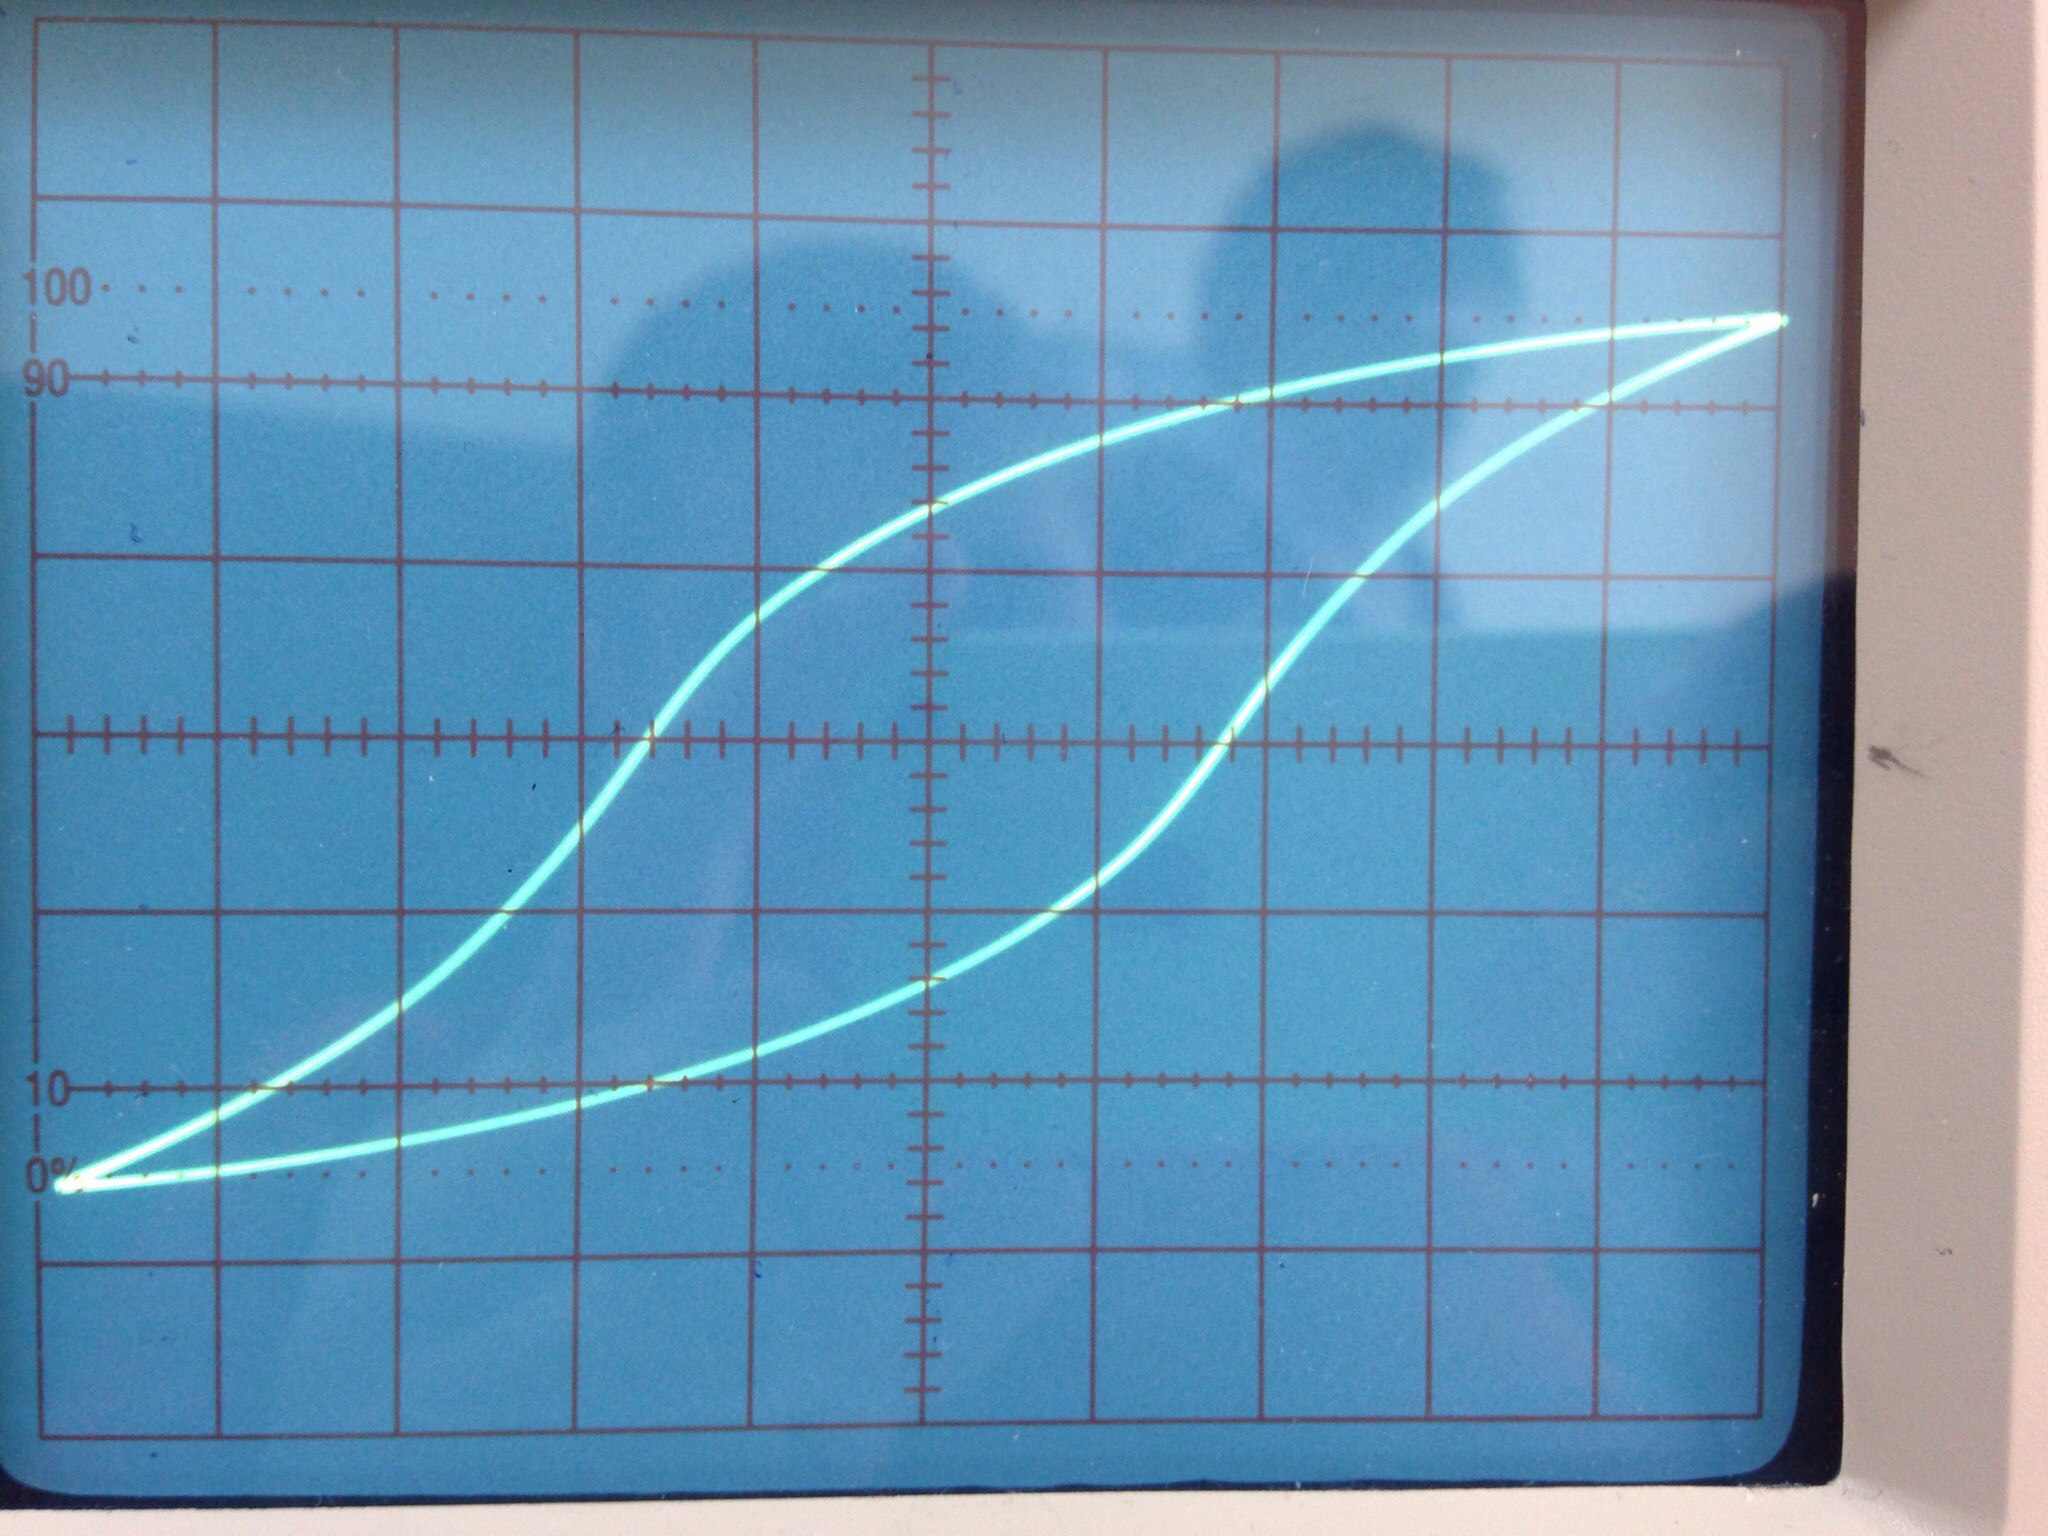
\includegraphics[width=\linewidth]{Fe-Si}}\\ предельная петля
	\end{minipage}
	\begin{minipage}[h]{0.5\linewidth}
		\center{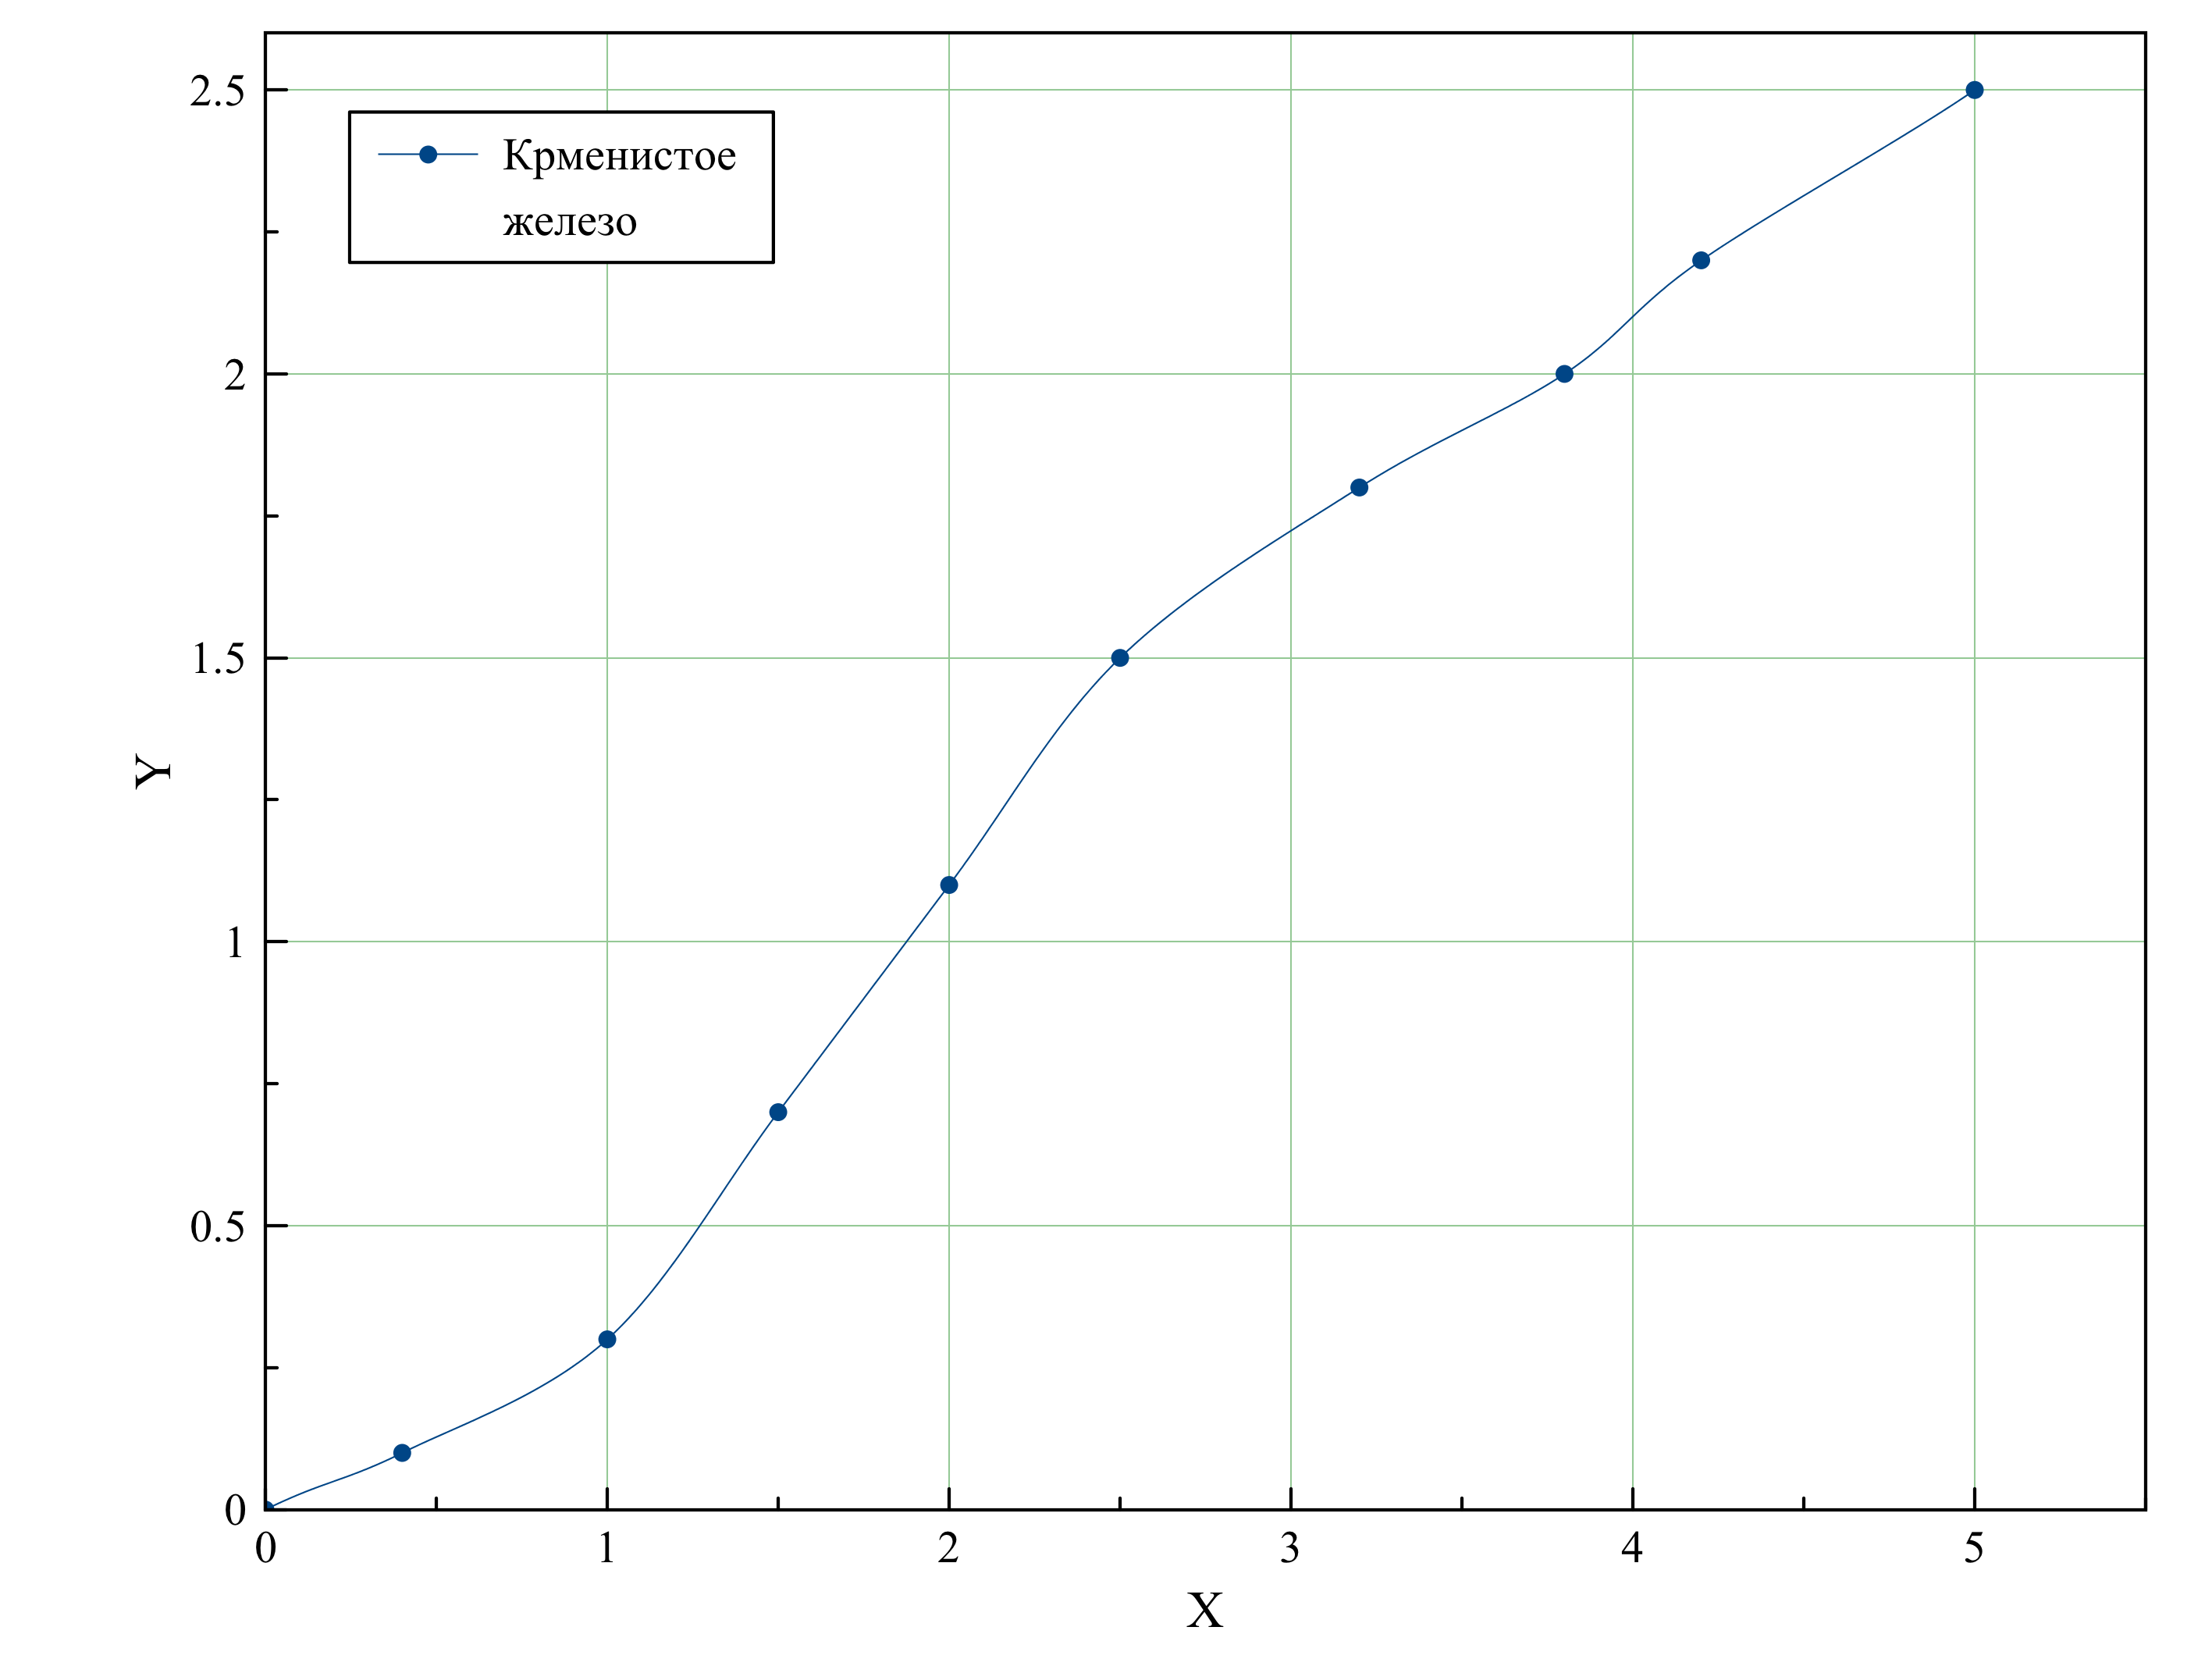
\includegraphics[width=\linewidth]{Fe-Si_plot}}\\ начальная кривая
	\end{minipage}
\end{figure}


\begin{center}
\textbf{2. Проверка калибровки оси X ЭО с помощью амперметра}
\end{center}

Отключим намагничивающую обмотку $N_0$ от цепи;  подберем такой ток через $R_0$ (с помощью реостата), при котором горизонтальная прямая занимает большую часть экрана; рассчитаем чувствительность канала $m_X$ по формуле и сравним с $K_X$. $2x=10$ делений.
$$m_x=\cfrac{2R_0\sqrt{2}I_{ef}}{(2x)}$$
\begin{itemize}
	\item Пермаллой: $m_x= 19.0 \text{ мВ} \approx K_X$
	\item Феррит: $m_x= 9.93 \text{ мВ} \approx K_X$
	\item Кремнистое железо: $m_x= 19.86 \text{ мВ} \approx K_X$
\end{itemize}

\newpage

\begin{center}
\textbf{3. Проверка калибровки оси Y ЭО с помощью вольтметра}
\end{center}

Разберем цепь тороида; подберем (с помощью реостата) напряжение, при котором вертикальная прямая занимает большую часть экрана; измерим двойную амплитуду сигнала; определим эффективное значение напряжения. $2y = 8$ делений.
$$m_y=\cfrac{2\sqrt{2}U_{ef}}{(2y)}$$
\begin{itemize}
	\item $K_Y=20 \text{ мВ/дел}; U_{ef}=139  \text{ мВ} \Rightarrow m_y = 49.1 \approx K_Y$
	\item $K_Y= 10 \text{ мВ/дел}; U_{ef}=27.3  \text{ мВ}\Rightarrow m_y = 9.7 \approx K_Y$
\end{itemize}


\begin{center}
\textbf{4. Определение $\tau$ - постоянной времени $RC$-цепочки}
\end{center}
Определим напряжения на входе и выходе интегрирующей ячейки: подключим $Y$-вход и отключим $X$-вход; установим чувствительность $K_Y \approx n$ В/дел; подберем такой ток (с помощью реостата), при котором горизонтальная прямая занимает большую часть экрана; определим входное напряжение на RC-цепочке; переключим $Y$-вход ЭО к интегрирующей емкости и определим $U_{ex}$; рассчитаем постоянную времени $\tau$
\begin{itemize}
	\item $K_Y =50 \text{ мВ/дел};~~ 2y=8;~~  U_{in}=2y\cdot K_Y=400 \text{ мВ}$
	\item $K_Y =50 \text{ мВ/дел};~~ 2y=0.4;~~ U_{ex}=2y\cdot K_Y=20 \text{ мВ}$
\end{itemize}

Имеем $\Omega=50$Гц; $\tau=R_uC_u=400 \text{ мс}$ $$~~~\tau=RC=\frac{U_{in}}{\Omega U_{ex}}=400 \text{мс}$$



\begin{center}
\textbf{5. Дифференциальная магнитная проницаемость}
\end{center}


Вычислим максимальные значения дифференциальной магнитной проницаемости  для каждого из трех образцов по формуле
$$\mu_{dif}=\frac{1}{\mu_0}\frac{dB}{dH},$$
где $\mu_0$ - магнитная постоянная ($\mu_0\approx1,256~ H/A^2$), а значение $\frac{dB}{dH}$ определим по графикам (максимальный наклон касательных к петлям гистерезиса, который достигается в точках с $B=0$, т.к. эти точки находятся наиболее далеко от областей насыщения). Также рассчитаем $H_c; B_s$ по формулам 
$$H=IN_0/(2\pi R);~~ B=R_u C_u U_{ex}/(SN_u);~~ U_{ex} = y\cdot K_Y$$
Результаты занесем в итоговую таблицу. 


\begin{table}[h]\centering
	\begin{tabular}{|m{3.3cm}|m{2.7cm}|m{2.7cm}|m{2.7cm}|}
		\hline
		~&Кремнистое железо&Пермаллой&Феррит\\
		\hline
		$H_c$, А/м&90.6$\pm$8.4&34.2$\pm$3.1&18.8$\pm$1.7\\
		\hline
		$B_s$, Тл&1.09$\pm$0.03&0.96$\pm$0.03&0.10$\pm$0.01\\
		\hline
		$\mu_{\text{дифф}}^{\max},~10^3$&9.8&50&2.7\\
		\hline
	\end{tabular}
\end{table}
\newpage
\section{Вывод}
Провели исследование петель гистерезиса трех ферромагнитных материалов(кремнистое железо, пермаллой и феррит). Для них мы построили начальные кривые гистерезиса для каждой из петель, нашли коэрцитивную силу и индукцию насыщения для каждого образца, оценили максимальные значения дифференциальной магнитной проницаемости для каждого образца, а также произвели калибровку осей ЭО и нашли постоянную $RC$-цепочки. Все экспериментально полученные результаты совпали с табличными кроме $H_c$ и $\mu_{\text{дифф}}^{\max}$ для Пермаллоя -- магнитная проницаемость достаточно меньше  табличного значения, вследствие чего, скорее всего не совпало и значения для $H_c$. Такое отклонение можно связать стем, что образец может быть довольно старым и изношенным, из-за чего у него и поменялись стандартные магнитные свойства. Полученные характеристики для данных материалов представляют практический интерес, т.к. часто используются в трансформаторах, дросселях, машинах переменного тока и пр.
\end{document}